\documentclass[11pt]{article}

\usepackage[utf8]{inputenc}
\usepackage[T1]{fontenc}
\usepackage{lmodern}
\usepackage[margin=1in]{geometry}
\usepackage{microtype}
\usepackage{amsmath,amssymb}
\usepackage{booktabs}
\usepackage{graphicx}
\usepackage{xcolor}
\usepackage{tikz}
\usetikzlibrary{arrows.meta,positioning,calc}
\usepackage{algorithm}
\usepackage{algpseudocode}
\usepackage{enumitem}
\usepackage{caption}
\usepackage[colorlinks=true,linkcolor=blue!50!black,citecolor=blue!50!black,urlcolor=blue!50!black]{hyperref}

\setlist{itemsep=2pt,topsep=3pt}
\setlength{\emergencystretch}{3em}
\captionsetup{font=small,labelfont=bf}
\newcommand{\unsat}{\textsf{unsat}}
\newcommand{\unknown}{\textsf{unknown}}
\newcommand{\timeout}{\textsf{timeout}}
\newcommand{\Q}{\mathcal{Q}}
\newcommand{\Cost}{\mathrm{cost}}

\title{\textbf{Spending Compute Where Proofs Are Fragile:\\
Budget-Aware Detection of SMT Instability on the Mariposa Benchmark}}
\author{Mohamed Ghoneim}
\date{October 2026}

\begin{document}
\maketitle

\begin{abstract}
SMT-based program verifiers are unstable: semantically irrelevant changes to a query, such as renaming symbols, reordering assertions or changing the solver's random seed, can turn a successful proof into a failure. Quantifying this instability is expensive because every query must be solved many times.
We ask a budgeted version of the question: given a fixed amount of solver CPU time and a collection of queries, \emph{in which order should equivalent variants be tested so that as many fragile queries as possible are exposed as early as possible?}
We formalise this task as \emph{budgeted witness search}, release an open pipeline that implements it, and compare four allocation strategies by replay on 268 queries from the Mariposa benchmark, measured with Z3~4.12.2 and a 10\,s timeout (8{,}744 solver runs, 9.8 CPU hours). Ground-truth labels come from independent reference variants never seen by the strategies, and strategy parameters are tuned on held-out projects.
A cost-aware Bayesian strategy beats uniform testing in all 20 replay seeds (area under the detection curve $0.833$ vs.\ $0.810$; paired difference $0.023$, 95\% interval over seeds $[0.013, 0.031]$) and reaches 80\% of the detectable fragile queries after 1.20 instead of 1.30 CPU hours; a simple runtime-priority heuristic is \emph{worse} than uniform testing. The gain is modest, it comes with slightly more flags that the reference labels do not corroborate, and with five project groups we cannot give a project-level confidence interval.
All 30 witness pairs we re-ran reproduced; two of them concern queries that recent work at EPFL diagnosed as a solver bug and a mis-set instantiation threshold.
We report the study as a careful, reproducible pilot rather than a definitive result, and list what would be needed to turn it into one.
\end{abstract}

%------------------------------------------------------------------------------
\section{Introduction}
\label{sec:intro}

Program verifiers such as Dafny~\cite{dafny}, F$^\star$~\cite{fstar} and Verus~\cite{verus} discharge verification conditions with SMT solvers such as Z3~\cite{z3} and cvc5~\cite{cvc5}. This automation makes verification practical for large systems~\cite{ironfleet,komodo,veribetrkv}, but it also makes it \emph{unstable}: a query that is solved in a second may fail, or time out, after a change that does not alter its meaning. The Mariposa study~\cite{mariposa} measured this on 17{,}043 queries from six verification projects and found that the newest solver it studied was unstable on 2.6\% of them, and on up to 5.0\% for individual projects.

Measuring instability is costly. Mariposa re-solves each query under many equivalent \emph{mutants}; the standard configuration used in follow-up work creates 180 mutants per query for a full stability test~\cite{cazamariposas}. For a project with thousands of queries, or for a continuous-integration setting, this is a substantial amount of solver time, much of it spent on queries that are consistently solved or consistently failed and therefore uninformative.

\paragraph{Question.} This report studies a deliberately narrow question. Suppose we only want to \emph{find} queries whose outcome depends on a harmless change, together with a concrete pair of equivalent variants that disagree (a \emph{witness}). Such a pair is exactly what downstream debugging tools consume: Cazamariposas~\cite{cazamariposas}, for instance, starts from one succeeding and one failing variant of an unstable query. Given a CPU budget $B$, how should we distribute tests across queries and variants to expose the most fragile queries as early as possible?

\paragraph{Approach.} We formalise the task as budgeted witness search (Section~\ref{sec:problem}), build a measurement and replay pipeline around it (Section~\ref{sec:method}), and evaluate four allocation strategies on a subset of the Mariposa benchmark (Sections~\ref{sec:setup} and~\ref{sec:results}). To avoid the usual trap of grading a detector on the same data it used to detect, labels come from \emph{independent} reference variants that no strategy can see, and strategy parameters are tuned on projects that are held out from evaluation.

\paragraph{Contributions.} We state them at the strength the evidence supports.
\begin{enumerate}
  \item \textbf{A problem formulation and evaluation protocol} for budgeted witness search: shared stopping rules so that strategies differ only in allocation, an independent pool/reference split of equivalent variants, held-out-project tuning, and metrics that express results as CPU time saved (Sections~\ref{sec:problem}--\ref{sec:method}).
  \item \textbf{An open, tested pipeline} (about 2{,}500 lines of Python plus 40 unit tests) containing a lossless SMT-LIB rewriter for the three Mariposa mutation families, a resumable measurement store with built-in noise controls, a replay evaluator, a live scheduler, and re-run confirmation with evidence bundles.
  \item \textbf{An empirical pilot on real data}: 268 queries, 8{,}744 solver runs. A cost-aware Bayesian allocation strategy finds fragile queries earlier than uniform, random and runtime-priority baselines; the improvement is small but consistent across seeds (Section~\ref{sec:results}).
  \item \textbf{Negative and null results that are useful to others}: a natural ``test the slow queries first'' heuristic is worse than uniform testing; project-level pooling, a slowness boost, and held-out tuning each fail to produce a measurable gain over the untuned core model; and part of the apparent early advantage over uniform testing is an artefact of its breadth-first schedule.
  \item \textbf{Validity evidence}: our labels agree strongly with the benchmark authors' own curated groups (none of the 81 curated-stable-core queries is labelled fragile, as expected from how that group was selected, while 45\% of curated-unstable queries are), identical-input noise is quantified (4 of 268 unchanged queries flip outcome), and all 30 witnesses re-run reproduced.
\end{enumerate}
We stress what this report is \emph{not}: it is a single-machine, single-solver-version, single-timeout study on five project groups. Section~\ref{sec:discussion} lists the threats to validity and the experiments that would address them.

%------------------------------------------------------------------------------
\section{Problem Statement}
\label{sec:problem}

\paragraph{Queries, variants, outcomes.}
Let $\Q$ be a set of SMT queries, each with exactly one \texttt{check-sat}, and let $T$ be a timeout. For a query $q$ and solver $s$, a \emph{variant} $v\in V(q)$ is either the original query or a meaning-preserving rewrite of it by one of three mutation families: \textbf{rename} (consistent renaming of declared symbols), \textbf{shuffle} (permuting consecutive assertions) or \textbf{reseed} (changing the solver's random seeds). These are the three mutations of Mariposa~\cite{mariposa,track}. Running $s$ on $(q,v)$ yields an outcome $o(q,v)\in\{\unsat,\textsf{sat},\unknown,\timeout,\textsf{memout}\}$ and a cost $\Cost(q,v)>0$, the CPU time of the solver process; a run that hits the timeout is charged the full $T$ so that budgets do not depend on machine load. A run is a \emph{success} if $o(q,v)=\unsat$ (a proof was found) and a \emph{failure} otherwise. Runs that end in a solver error are not failures; they are discarded and reported.

\paragraph{Witnesses.}
A \emph{witness} for $q$ is a pair of variants $(v,v')$ with $o(q,v)$ a success and $o(q,v')$ a failure. We say $q$ is \emph{flagged} once a witness has been observed. A witness is a certificate that the outcome of $q$ depends on a harmless change, up to measurement noise, which we control by re-running witnesses (Section~\ref{sec:confirm}).

\paragraph{Budgeted witness search.}
Given a budget $B$ of solver CPU time, a strategy sequentially chooses $(q,v)$ pairs to test, observes the outcome and cost, and may stop testing a query at any time. Its goal is to maximise the number of fragile queries flagged within budget $B$, for every $B$ simultaneously; equivalently, to make the detection curve rise as early as possible.

\paragraph{Independent reference labels.}
To score a strategy we need to know which queries are truly sensitive. We split the measured variants of each query into a \emph{pool} $P_q$ (the original and the variants with even index) and an independent \emph{reference} set $R_q$ (the variants with odd index). Strategies may only test pool variants. The label of $q$ is computed from the reference success rate $\hat p_q = |\{v\in R_q: \text{success}\}|/|R_q|$:
\begin{equation}
\mathrm{label}(q)=\begin{cases}
\textit{pure} & \hat p_q\in\{0,1\},\\
\textit{fragile} & \delta\le \hat p_q\le 1-\delta,\\
\textit{borderline} & \text{otherwise},
\end{cases}\qquad \delta=0.1 .
\end{equation}
With about 15 reference variants per query, \emph{fragile} means roughly at least two successes and two failures. A flag on a \emph{pure} query is not necessarily an error (a query that succeeds on 5\% of variants will often look pure in 15 reference runs), so we call such flags \emph{uncorroborated}. The \emph{ceiling} is the number of fragile queries that would be flagged if the entire pool were tested; recall is measured against it.

\paragraph{Metric.}
Let $b\in[0,1]$ be the budget as a fraction of the cost of testing every pool variant of every query ($4.72$ CPU hours in our data), and $R(b)$ the recall of fragile queries at budget $b$. We summarise a strategy by $\mathrm{AUDC}=\int_0^1 R(b)\,db$, the area under the detection curve. Because both curves are monotone and reach 1, the difference of two AUDCs equals the CPU-time saving averaged uniformly over recall levels, expressed as a fraction of the exhaustive cost; we also report the CPU hours needed to reach fixed recall levels, which is easier to interpret.

%------------------------------------------------------------------------------
\section{Method}
\label{sec:method}

Figure~\ref{fig:pipeline} gives an overview of the pipeline.

\begin{figure}[t]
\centering
\resizebox{\textwidth}{!}{%
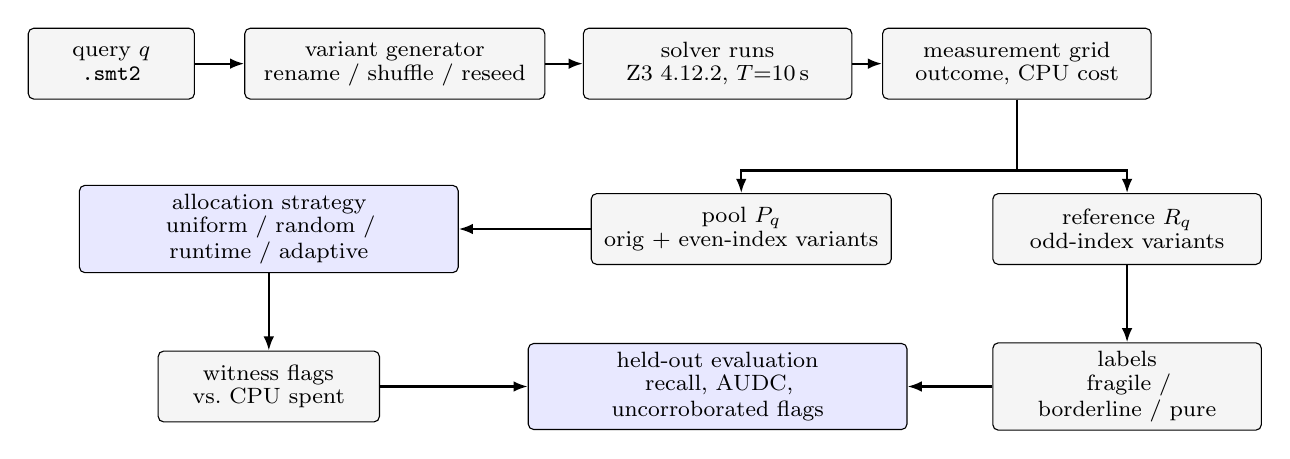
\begin{tikzpicture}[
  box/.style={draw, rounded corners=2pt, align=center, font=\footnotesize, minimum height=9mm, inner sep=3pt, fill=gray!8},
  hl/.style={draw, rounded corners=2pt, align=center, font=\footnotesize, minimum height=9mm, inner sep=3pt, fill=blue!9},
  arr/.style={-{Latex[length=1.8mm]}, thick}]
\node[box, text width=1.9cm] (q) at (0,0) {query $q$\\[-1pt]\texttt{.smt2}};
\node[box, text width=3.6cm] (v) at (3.6,0) {variant generator\\[-1pt]rename / shuffle / reseed};
\node[box, text width=3.2cm] (s) at (7.7,0) {solver runs\\[-1pt]Z3 4.12.2, $T{=}10$\,s};
\node[box, text width=3.2cm] (g) at (11.5,0) {measurement grid\\[-1pt]outcome, CPU cost};
\node[hl, text width=4.6cm] (strat) at (2.0,-2.1) {allocation strategy\\[-1pt]uniform / random / runtime / adaptive};
\node[box, text width=3.6cm] (pool) at (8.0,-2.1) {pool $P_q$\\[-1pt]orig + \mbox{even-index} variants};
\node[box, text width=3.2cm] (ref) at (12.9,-2.1) {reference $R_q$\\[-1pt]odd-index variants};
\node[box, text width=2.6cm] (flags) at (2.0,-4.1) {witness flags\\[-1pt]vs.\ CPU spent};
\node[hl, text width=4.6cm] (eval) at (7.7,-4.1) {held-out evaluation\\[-1pt]recall, AUDC, \mbox{uncorroborated} flags};
\node[box, text width=3.2cm] (lab) at (12.9,-4.1) {labels\\[-1pt]fragile / \mbox{borderline} / pure};
\draw[arr] (q) -- (v); \draw[arr] (v) -- (s); \draw[arr] (s) -- (g);
\draw[arr] (g.south) -- ++(0,-0.9) -| (pool.north);
\draw[arr] (g.south) -- ++(0,-0.9) -| (ref.north);
\draw[arr] (pool.west) -- (strat.east);
\draw[arr] (strat) -- (flags);
\draw[arr] (ref) -- (lab);
\draw[arr] (flags.east) -- (eval.west);
\draw[arr] (lab.west) -- (eval.east);
\end{tikzpicture}}
\caption{Pipeline. Every query is measured once on all its variants. Strategies are replayed on the recorded \emph{pool} measurements only; ground-truth labels come from the independent \emph{reference} measurements.}
\label{fig:pipeline}
\end{figure}

\subsection{Meaning-preserving variants}
\label{sec:variants}

We implemented the three Mariposa mutation families ourselves, in a form that never interprets a query beyond its command structure.

\textbf{Lossless splitting.} A script is split into top-level commands and the trivia (spaces, comments) between them, such that concatenating the pieces reproduces the file exactly. This holds for strings with escaped quotes and for quoted symbols \texttt{|...|}.

\textbf{rename.} The symbols \emph{declared by the script itself} (via \texttt{declare-fun}, \texttt{declare-const}, \texttt{define-fun}, \texttt{define-fun-rec}, \texttt{define-const}, \texttt{declare-sort}, \texttt{define-sort}) are mapped by an injective function to fresh names (a 40-bit random suffix, checked to be unused in the file) and replaced at the token level everywhere except inside strings and comments. Because the mapping is injective on tokens and the new names are fresh, this is an $\alpha$-renaming of the declared signature.

\textbf{shuffle.} Maximal runs of \emph{consecutive} \texttt{assert} commands (only trivia in between) are permuted. Assertions are never moved across a declaration, \texttt{push}, \texttt{pop} or \texttt{check-sat}, so scoping is preserved, and the conjunction of the assertions in a run is commutative.

\textbf{reseed.} The text is unchanged and the solver is run with \texttt{smt.random\_seed} and \texttt{sat.random\_seed} set to a derived value.

Every variant is a deterministic function of (base seed, query id, variant id), so it can be regenerated later for evidence bundles. A family is only planned for a query if it can change it (e.g., no shuffle when no run of two assertions exists), which avoids duplicate runs. Unit tests check losslessness, round-trip renaming, that strings and comments are untouched, that assertions never cross boundaries, and determinism; on the real data every variant but one was accepted by the solver (Section~\ref{sec:results}). These rewrites are an independent re-implementation, not the Mariposa mutator, so our mutants are not identical to Mariposa's.

\subsection{Measurement protocol}
\label{sec:measure}

Each solver run writes the variant to a temporary file and invokes \texttt{z3 -smt2 -T:10 -memory:3000} (plus the seed options for reseeded variants) as a child process. We record the outcome of the \emph{first} \texttt{check-sat} (later error lines such as a \texttt{get-model} after \unsat{} are ignored), wall time, and the child's CPU time. A hit of the memory limit is reported by Z3 as \texttt{(error "out of memory")}, on standard error in the version we use, and is recorded as \textsf{memout}, a failure. Runs are executed by four worker processes on a 16-thread machine, and the load average is recorded with every run. Every query is measured on all its planned variants (up to 31: the original plus 10 variants per family), and the original is re-run twice more as a noise control. The store is an append-only log, so interrupted runs resume.

\subsection{Allocation strategies}
\label{sec:strategies}

All strategies answer one question, \emph{which query receives the next test?}, and share the following rules, so that they differ only in allocation: (i) the variant tested next is the next one in the query's seeded random order, with the original first; (ii) a flagged query is never tested again; (iii) a query whose pool is exhausted is never tested again; (iv) all strategies see identical variant orders for the same replay seed (a paired design). Algorithm~\ref{alg:search} shows the common loop.

\begin{algorithm}[t]
\caption{Budgeted witness search (shared by all strategies)}
\label{alg:search}
\begin{algorithmic}[1]
\Require queries $\Q$, variant order $\sigma_q$ for each $q$ (original first), budget $B$, strategy $\pi$
\State $n_q,s_q,f_q\gets 0$ for all $q$;\; $\mathrm{spent}\gets 0$;\; $\mathcal{F}\gets\emptyset$
\While{$\mathrm{spent}<B$ \textbf{and} some query is eligible \Comment{$q\notin\mathcal F$ and $n_q<|P_q|$}}
  \State $q\gets \pi.\mathrm{pick}()$
  \State $v\gets\sigma_q[n_q]$;\; run the solver on $(q,v)$;\; observe success $y$ and cost $c$
  \State $\mathrm{spent}\gets \mathrm{spent}+c$;\; $n_q\gets n_q+1$;\; increment $s_q$ if $y$ else $f_q$;\; $\pi.\mathrm{update}(q,y,c)$
  \If{$s_q>0$ \textbf{and} $f_q>0$} $\mathcal F\gets\mathcal F\cup\{q\}$ \EndIf
\EndWhile
\State \Return $\mathcal F$ with a witness pair for each flagged query
\end{algorithmic}
\end{algorithm}

\paragraph{Uniform} is breadth-first: it always tests a query with the fewest tests so far. \textbf{Random} picks uniformly among the remaining (query, variant) pairs. \textbf{Runtime-priority} is a simple heuristic that a practitioner might try: after two warm-up tests per query it prefers queries that were solved but slowly (largest successful cost divided by $T$); queries that never succeeded come last.

\paragraph{Adaptive.} The adaptive strategy scores each query by the estimated probability that its next test creates a witness, per expected CPU second, and mixes in a small amount of exploration. It is a heuristic built on an explicit, simple model; the model's assumptions are not claimed to be true and are exactly what the experiment probes. After a warm-up of $k_0=2$ tests per query (random order), a query with $n$ unanimous outcomes is scored as follows.

\begin{itemize}
  \item Each query is \emph{mixed} with prior probability $\pi_j$ (project $j$) and otherwise \emph{pure} (always succeeds or always fails). A mixed query succeeds on each variant with probability $\theta\sim\mathrm{Beta}(a,b)$, $a=b=2$.
  \item The marginal likelihood of $n$ unanimous successes under a mixed query is $L_s(n)=B(a{+}n,b)/B(a,b)$; for $n$ unanimous failures it is $L_f(n)=B(a,b{+}n)/B(a,b)$. By Bayes' rule the posterior odds that the query is mixed are
  \begin{equation}
  \frac{P(\text{mixed}\mid\text{data})}{P(\text{pure}\mid\text{data})}
  =\frac{\pi_j}{1-\pi_j}\cdot\frac{L(n)}{\rho}\cdot\bigl(1+\gamma\, m_q/T\bigr),
  \end{equation}
  where $\rho$ is the (online-estimated) share of unanimous queries on the observed side, and $m_q$ is the slowest successful cost of $q$, so that queries solved only slowly get their odds multiplied by $1+\gamma m_q/T$ ($\gamma$ is a hyper-parameter; $\gamma{=}0$ disables the boost).
  \item The probability that the next test reveals the opposite outcome is $P(\text{mixed}\mid\text{data})\cdot b/(a{+}b{+}n)$ after unanimous successes and $\cdot\,a/(a{+}b{+}n)$ after unanimous failures.
  \item The expected cost of the next test is $\hat c_q=(C_q+c_0\bar c_j)/(n_q+c_0)$, where $C_q$ is the cost spent on $q$, $\bar c_j$ the observed mean cost per test in project $j$, and $c_0=1$.
  \item The \emph{score} is the revealing probability divided by $\hat c_q$. With probability $\varepsilon$ a step is instead an \emph{exploration} step on the least-tested eligible query.
  \item The project prior $\pi_j=(F_j+\kappa\bar\pi)/(W_j+\kappa)$ is shrunk toward the global rate $\bar\pi=(F+20\pi_0)/(W+20)$, where $F_j$ is the number of flagged queries and $W_j$ the number of warmed-up queries in project $j$ so far, $\pi_0=0.05$, and $\kappa$ is a hyper-parameter. Project-level statistics are refreshed every 100 steps; per-query scores are updated after every test in constant time.
\end{itemize}
No ground-truth labels are used; the strategy only sees outcomes and costs observed so far. The defaults are $\varepsilon=0.1$, $\gamma=2$, $\kappa=10$.

\subsection{Evaluation protocol}
\label{sec:protocol}

Strategies are evaluated by \emph{replay}: the measurement grid is recorded once, and each strategy is run on it for 20 replay seeds, each seed fixing the per-query variant orders (shared by all strategies) and the strategy's own randomness. The projects are split into three folds. For each fold, the \emph{tuned} adaptive strategy selects $(\varepsilon,\gamma,\kappa)$ from a grid of $2\times2\times2$ values by maximising AUDC on the \emph{training} projects (three seeds) and is then evaluated on the held-out projects; queries of one project are never split between training and evaluation. Curves from the folds are pooled on the fractional-budget axis. The analysis plan, including the primary comparison (tuned adaptive vs.\ uniform, $\delta=0.1$, independent labels) and the commitment to report the outcome even if the adaptive strategy does not win, was written down before the real measurements were collected, and the evaluation was run once on the real data. The strategies and code were developed and tested only on synthetic data produced by a mock solver.

\subsection{Re-running witnesses}
\label{sec:confirm}

A witness can be a measurement artefact, especially near the timeout. For a set of witnesses we regenerate the two variants from their specification, re-run each side five times, and call the witness \emph{reproduced} if both sides give the recorded success/failure status in at least four of five runs. Reproduced witnesses are written as evidence bundles containing both \texttt{.smt2} files and a shell script that re-runs them.

%------------------------------------------------------------------------------
\section{Experimental Setup}
\label{sec:setup}

\paragraph{Data.} We use the Mariposa benchmark~\cite{mariposa}, a collection of 935 queries from six verification projects (Komodo$_D$ and Komodo$_S$~\cite{komodo}, two variants of VeriBetrKV~\cite{veribetrkv}, DICE$^\star_F$~\cite{dice} and vWasm$_F$~\cite{vwasm}), which its authors classified into four curated groups: \emph{unstable core} (unstable under both an older and the then-latest Z3), \emph{unstable extension} (further queries unstable under Z3 4.12.1), \emph{stable core} (30 random stable queries per project with runtime standard deviation under one second) and \emph{stable extension} (stable queries with standard deviation above six seconds). The authors used a 60\,s timeout. The benchmark is therefore \emph{enriched} for unstable queries by construction and does not reflect natural prevalence.

We drew a random sample of up to 60 queries per project group (seed 0), balanced across groups, and excluded one 23.1\,MB query (size cap 20\,MB). The result is 268 queries in five project groups: dice (55), fvbkv (59), komodo (60), lvbkv (60) and vwasm (34). Project groups were inferred from file names; Komodo$_D$ and Komodo$_S$ are consequently pooled, and the two VeriBetrKV variants are kept separate. By curated group, the sample contains 81 stable-core, 85 stable-extension, 14 unstable-core and 88 unstable-extension queries.

\paragraph{Environment.} Z3 4.12.2 (the \texttt{z3-solver} 4.12.2.0 package), timeout $T=10$\,s, memory limit 3000\,MB per run, on an AMD Ryzen 7 6800H laptop (16 hardware threads), four workers, laptop plugged in; the median load average was 4.0. The 8{,}744 distinct measurements were collected under Ubuntu 22.04 (Linux 6.8.0-138, glibc 2.35, Python 3.10.12); the main run took about 2.4 hours of wall time, plus a 13-minute pilot. The laptop was later upgraded to Ubuntu 24.04 (Linux 6.8.0-147, glibc 2.39, Python 3.12.3) with the same Z3 4.12.2 package; the single re-measurement described in Section~\ref{sec:results}, the evaluation and the witness re-runs were performed in that environment. The 268 queries were measured on 8{,}208 planned variant runs plus 536 control repeats, i.e.\ 8{,}744 distinct measurements (8{,}745 log lines, because one record was superseded) and 9.76 solver CPU hours (timeouts charged in full). We chose a 10\,s timeout, shorter than the 60\,s used to curate the benchmark, to keep the study within a laptop budget; this affects labels (Section~\ref{sec:discussion}).

%------------------------------------------------------------------------------
\section{Results}
\label{sec:results}

\subsection{Measurement outcomes and validity checks}

Of the 8{,}208 planned runs, 5{,}608 (68.3\%) ended in \unsat, 2{,}353 (28.7\%) in \timeout, 246 (3.0\%) in \unknown{} and one (0.01\%) in \textsf{memout}. The \textsf{memout} is a renamed variant (\texttt{rename:8}) of a stable-extension Komodo query: Z3 stopped after 5.7\,s of CPU time with \texttt{(error "out of memory")} on standard error, whereas the same variant run without the memory limit times out after 10\,s, and the original query also times out. This run was first recorded as a solver error, because our output parser inspected only standard output, and since errors are excluded from the analysis it was initially dropped. We found the cause by re-running the variant, fixed the parser, added a regression test, and re-measured the run with the corrected code; the superseded record remains in the log. All numbers in this report use the corrected data. The correction changed no AUDC value by more than 0.002 and no qualitative conclusion. No run returned \textsf{sat}, so no pair of equivalent variants contradicted each other; a \textsf{sat}/\unsat{} disagreement would have indicated either a solver soundness bug or a defect in our rewrites.

\paragraph{Noise on identical input.} Of the 268 unchanged originals, each run three times, 4 (1.5\%) changed success/failure status; the median relative runtime spread among repeated successful runs (for queries whose fastest run exceeded 0.05\,s) was 5.1\% (95th percentile 20.7\%). This is the floor on spurious witnesses caused by timing near the timeout alone.

\paragraph{Labels.} The independent reference labels 66 queries (24.6\%) \emph{fragile}, 25 (9.3\%) \emph{borderline} and 177 (66.0\%) \emph{pure}. Of the 66 fragile queries, 61 are detectable from the pool (the ceiling); 16 pure and 12 borderline queries also show a witness somewhere in the pool.

\begin{figure}[t]
\centering
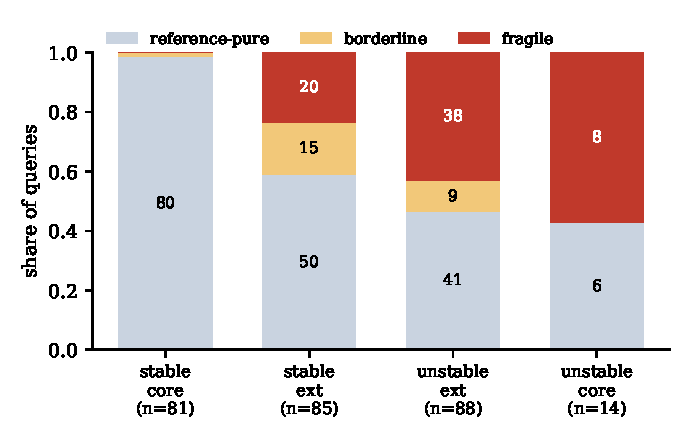
\includegraphics[width=0.62\textwidth]{figs/fig_groups.pdf}
\caption{Agreement between our independent reference labels and the benchmark authors' curated groups (counts inside bars). Of 81 stable-core queries, none is labelled fragile and one borderline; 57\% of unstable-core queries are fragile. Six unstable-core queries are labelled pure at our 10\,s timeout.}
\label{fig:groups}
\end{figure}

\paragraph{Agreement with the curated groups.} Figure~\ref{fig:groups} compares our labels with the authors' groups, which we did not use anywhere in the pipeline. The fragile share is 0\% (0/81) for stable core, 24\% (20/85) for stable extension, 43\% (38/88) for unstable extension and 57\% (8/14) for unstable core; pooled, 45\% (46/102) of curated-unstable queries are fragile against 12\% (20/166) of curated-stable ones. These are descriptive counts: queries from one project are not independent, so we do not attach a significance test. The zero for stable core is a sanity check rather than evidence of discriminative power, since those queries were selected for run-time standard deviation below one second. The contrast between the unstable groups (43--57\%) and the overall stable pool (12\%) is the more informative result. The agreement is not perfect, as expected from different solver builds and a 6$\times$ shorter timeout. The 20 fragile stable-extension queries are consistent with that group's definition (stable by average, but with large runtime variance).

\subsection{Main comparison}

Table~\ref{tab:main} and Figure~\ref{fig:main} summarise the comparison. Exhaustively testing every pool variant of every query would cost 4.72 CPU hours; all strategies stop testing a query after a witness, so all of them reach 80\% recall at 26--38\% of that cost. That saving is due to the shared stopping rules, not to any allocation strategy.

\begin{table}[t]
\centering
\caption{Main results (268 queries, five project groups; tuned strategy evaluated on held-out projects). AUDC: mean and 2.5--97.5 percentile over 20 replay seeds. Hours: solver CPU hours to reach the recall level on the seed-averaged curve (exhaustive pool testing: 4.72\,h). Recall at 10\% and 25\% of the exhaustive budget (0.47\,h and 1.18\,h).}
\label{tab:main}
\footnotesize
\setlength{\tabcolsep}{4pt}
\begin{tabular}{lcccccc}
\toprule
strategy & AUDC & h to 50\% & h to 80\% & h to 90\% & recall @10\% & recall @25\%\\
\midrule
uniform & 0.810 [0.785, 0.840] & 0.76 & 1.30 & 1.68 & 0.22 & 0.76\\
random & 0.803 [0.768, 0.838] & 0.83 & 1.39 & 1.77 & 0.25 & 0.72\\
runtime-priority & 0.779 [0.756, 0.812] & 0.87 & 1.77 & 2.31 & 0.33 & 0.64\\
adaptive (defaults) & \textbf{0.835} [0.813, 0.863] & \textbf{0.66} & \textbf{1.20} & \textbf{1.53} & 0.31 & \textbf{0.80}\\
adaptive (tuned) & 0.833 [0.813, 0.861] & \textbf{0.66} & \textbf{1.20} & 1.58 & 0.32 & \textbf{0.80}\\
\bottomrule
\end{tabular}
\end{table}

\begin{figure}[t]
\centering
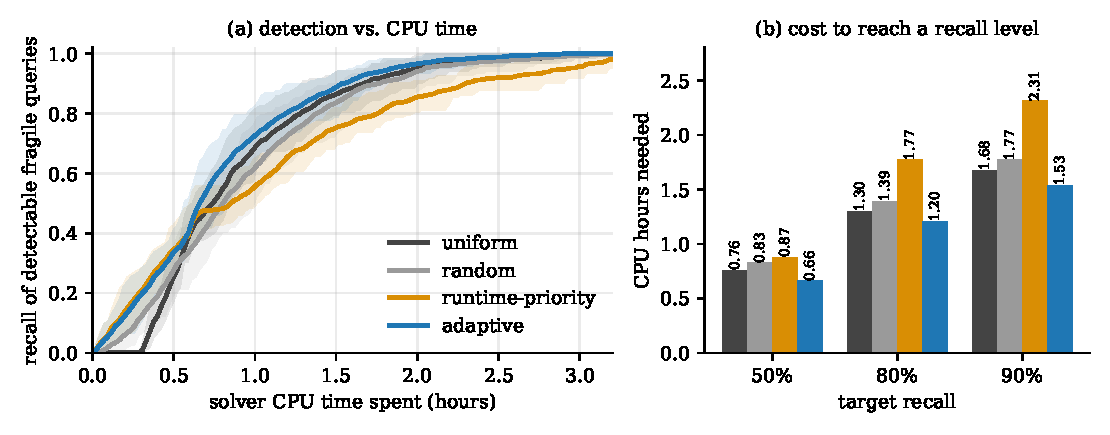
\includegraphics[width=\textwidth]{figs/fig_main.pdf}
\caption{(a) Recall of detectable fragile queries against solver CPU time; bands show the 2.5--97.5 percentile over 20 replay seeds. (b) CPU hours needed to reach 50\%, 80\% and 90\% recall.}
\label{fig:main}
\end{figure}

\paragraph{Primary comparison.} The pre-specified comparison, tuned adaptive vs.\ uniform, gives an AUDC difference of $+0.023$ (95\% interval over seeds $[0.013, 0.031]$), and the adaptive strategy is better in 20 of 20 seeds (untuned defaults: $+0.025$, $[0.014, 0.033]$, 20/20). Since both curves reach 1, this corresponds to saving roughly $0.023\times4.72\approx0.11$ CPU hours on average over recall levels, about 6.5 minutes. At fixed recall the saving is $12\%$ (50\%), $7\%$ (80\%) and $8\%$ (90\%) of uniform's CPU time for the untuned model. Runtime-priority is worse than uniform ($-0.032$, $[-0.054,-0.011]$, better in 0/20 seeds); random is indistinguishable from uniform ($-0.007$, $[-0.025, 0.006]$, 5/20). The adaptive strategy's AUDC exceeds random's by 0.032 and runtime-priority's by 0.057 (means only; we did not compute paired intervals for these).

\paragraph{How much of the early advantage is real?} At 5\% of the budget uniform has flagged nothing: its breadth-first schedule gives every query a first test before any query gets a second, so it cannot form a witness during the first $\approx$0.3 CPU hours (Figure~\ref{fig:main}a). Random, which has no such delay, is already at 0.25 recall at 10\%, above uniform's 0.22. We therefore regard the gap at very small budgets as largely a property of the baseline's schedule. The more informative differences appear at mid budgets, where all strategies have passed their warm-up: recall at 15\% / 25\% / 40\% of the budget is $0.55$ / $0.80$ / $0.96$ for adaptive against $0.48$ / $0.76$ / $0.94$ for uniform.

\subsection{Ablations and tuning}

\begin{figure}[t]
\centering
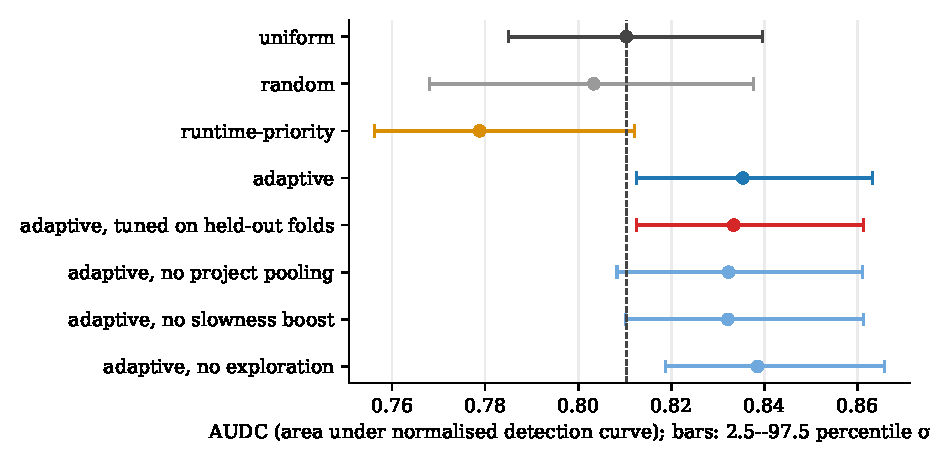
\includegraphics[width=0.78\textwidth]{figs/fig_audc.pdf}
\caption{AUDC for every strategy and ablation (dashed line: uniform). Differences among the adaptive variants are far smaller than their separation from uniform and runtime-priority, and well within the seed-to-seed spread.}
\label{fig:audc}
\end{figure}

Figure~\ref{fig:audc} and Table~\ref{tab:ablation} show that removing project-level pooling ($0.832$), removing the slowness boost ($0.832$) or removing exploration ($0.839$) leaves AUDC essentially unchanged (all within $0.003$ of the default $0.835$), and tuning on held-out projects does not improve it ($0.833$). The tuned parameters differ between folds ($\gamma=3,0,3$; $\kappa=25,5,5$; $\varepsilon=0.05$ throughout), which indicates a flat optimum on this data. We conclude that, on this benchmark subset, the benefit comes from the common core of the model (the Bayesian probability of revealing a witness divided by expected cost), and that the additional components are not shown to matter. We did not run an ablation that removes the cost term, so we cannot say how much of the gain is attributable to cost-awareness as opposed to the Bayesian ranking.

\begin{table}[t]
\centering
\caption{Paired AUDC difference to uniform over 20 replay seeds (percentile interval over seeds) and number of seeds in which the strategy is better.}
\label{tab:ablation}
\small
\begin{tabular}{lccc}
\toprule
strategy & AUDC & difference to uniform & seeds better\\
\midrule
random & 0.803 & $-$0.007 [$-$0.025, +0.006] & 5/20\\
runtime-priority & 0.779 & $-$0.032 [$-$0.054, $-$0.011] & 0/20\\
adaptive (defaults) & 0.835 & +0.025 [+0.014, +0.033] & 20/20\\
adaptive (tuned) & 0.833 & +0.023 [+0.013, +0.031] & 20/20\\
\ \ no project pooling & 0.832 & +0.022 [+0.012, +0.030] & 20/20\\
\ \ no slowness boost & 0.832 & +0.022 [+0.010, +0.031] & 20/20\\
\ \ no exploration & 0.839 & +0.028 [+0.017, +0.037] & 20/20\\
\bottomrule
\end{tabular}
\end{table}

\subsection{What the extra detections cost: uncorroborated flags}

Finding witnesses faster is only useful if the flagged queries are genuinely sensitive. Table~\ref{tab:flags} decomposes the flags at 25\% of the budget by reference label. The adaptive strategy flags more queries overall (63 vs.\ 56 for uniform) and more fragile ones (48.6 vs.\ 46.5), but also more that the reference does not call fragile, so its label precision at this budget is lower (77\% vs.\ 83\%). Runtime-priority has the lowest precision (71\%). At 10\% of the budget precision is similar for adaptive, uniform and runtime-priority (88\%, 86\%, 88\%). Because ``pure'' flags may be rare-event witnesses rather than errors, this is not necessarily a defect, but it means the strategy's advantage in finding fragile queries is partly paid for by flagging queries on the fragility boundary. Every strategy eventually flags all 16 flaggable pure queries (the maximum possible).

\begin{table}[t]
\centering
\caption{Composition of flagged queries at 25\% of the exhaustive budget (mean over seeds): reference label of each flagged query and label precision (fragile / all flagged).}
\label{tab:flags}
\small
\begin{tabular}{lccccc}
\toprule
strategy & fragile & borderline & pure (uncorroborated) & all flagged & precision\\
\midrule
uniform & 46.5 & 4.2 & 5.1 & 55.7 & 0.83\\
random & 43.7 & 4.3 & 5.4 & 53.4 & 0.82\\
runtime-priority & 39.2 & 7.6 & 8.8 & 55.6 & 0.71\\
adaptive (defaults) & 48.6 & 7.7 & 6.8 & 63.1 & 0.77\\
adaptive (tuned) & 48.5 & 8.1 & 7.5 & 64.1 & 0.76\\
\bottomrule
\end{tabular}
\end{table}

\subsection{Witnesses re-run and examples}

We re-ran the 30 cheapest witnesses (cheapest first, to keep the confirmation affordable) five times per side. All 30 reproduced in all five runs on both sides. They comprise 18 unstable-extension, 7 unstable-core and 5 stable-extension queries from four project groups (fvbkv 15, lvbkv 11, vwasm 3, komodo 1). In every pair the original query is one side. The original succeeded and a variant failed in 20 pairs (12 \unknown, 8 \timeout) and the reverse in 10 (8 \unknown, 2 \timeout); the other side was a renamed variant in 22 pairs, a shuffled one in 6 and a reseeded one in 2. These counts are descriptive only: witnesses were selected cheapest first, which favours quick \unknown{} failures (20 of 30) over slow timeouts, and the variant paired with the original was the cheapest opposite-outcome variant. The split between quick \unknown{} and slow \timeout{} failures matches the two failure modes described by Zhou et al.~\cite{cazamariposas}. Reproduction demonstrates that a witness is not timing noise on this machine; it does not explain \emph{why} the solver behaves differently.

Two of the 30 queries are among the 11 unstable queries whose root causes were analysed by Cebeci et al.~\cite{conjecture} (using Z3 builds between 4.13.4 and 4.14.2): \texttt{lemma\_2toX}, which they attribute to a too-small quantifier-instantiation threshold, and \texttt{set\_bit\_to\_0\_self\_uint64}, which they attribute to a solver bug fixed upstream. In our runs, the original of \texttt{lemma\_2toX} returns \unknown{} and a shuffled variant returns \unsat; the original of \texttt{set\_bit\_to\_0\_self\_uint64} times out and a renamed variant returns \unsat, each reproduced five times with Z3 4.12.2. This shows that our pipeline surfaces queries that expert analysis independently identified as unstable; we make no claim about whether the same root causes are responsible in Z3 4.12.2.

%------------------------------------------------------------------------------
\section{Discussion and Threats to Validity}
\label{sec:discussion}

\paragraph{What the data support.} On this subset, a cost-aware Bayesian allocation finds fragile queries somewhat earlier than uniform or random testing, and a runtime-priority rule is worse than uniform. The practical effect is small (on the order of 7--12\% of the CPU time needed to reach a given recall), consistent across replay seeds, and accompanied by more uncorroborated flags. The main saving over exhaustive testing comes from stopping once a witness is found, which every strategy does.

\paragraph{What they do not support.} We do not claim that the adaptive strategy is superior in general, that its model is correct (the ablations show that three of its components are not needed for the observed gain), or that the effect would hold on other solvers, timeouts or query distributions.

\paragraph{Statistical limits.} The intervals reflect randomness of variant order and exploration over 20 replay seeds. They do not reflect the sampling of queries or projects. With five project groups, a project-level bootstrap is not meaningful (our tool requires at least eight), so we do not provide one; the evidence is for this benchmark subset, not for a population of verification queries. We ran one pre-specified comparison and report all variants we ran, with no correction for multiple comparisons; the label-threshold and label-mode sensitivity analyses in our plan ($\delta\in\{0.05,0.2\}$; labels from pool and reference together) were not run for this report.

\paragraph{Construct validity.} Our notion of fragility (a witness pair, labelled by the reference success rate in $[\delta,1-\delta]$) is not Mariposa's statistical stability test, and our labels depend on the timeout, as do existing metrics, a limitation emphasised by Cebeci et al.~\cite{conjecture}: at 10\,s some queries that need longer appear as pure failures (six of the 14 unstable-core queries), while at 60\,s other queries would look stable. Reference labels are estimated from about 15 variants and have sampling error themselves, so some ``uncorroborated'' flags may be real but rare. Our rewrites are our own implementation of the three mutation families and may differ from Mariposa's mutants.

\paragraph{Internal validity.} Replay evaluates strategies on a recorded grid and not live; identical-input runs flip in 1.5\% of queries, so some witnesses near the timeout can be noise (the re-runs argue against this for the 30 we checked, but they were the cheapest, not a random sample). The strategies cannot adapt which variant of a query to test, only which query. One run, a memory-limit hit, was initially misclassified by our output parser and corrected after we diagnosed it (Section~\ref{sec:results}). The measurements were taken under Ubuntu 22.04 and the corrected run, the evaluation and the witness re-runs under Ubuntu 24.04 with the same Z3 package; the witness pairs, whose outcomes had been recorded under the older system, reproduced after the upgrade. Four workers share one laptop; timings carry the corresponding noise (median relative spread 5\%).

\paragraph{External validity.} One benchmark enriched for unstable queries; Z3 4.12.2 only; one timeout; five project groups with Komodo$_D$ and Komodo$_S$ pooled; one hardware platform. Queries from a newer Z3 with improved generation accounting~\cite{depth} may show different instability profiles.

\paragraph{What would settle it.} (i) More projects, e.g.\ the Verus query sets curated by the Mariposa authors~\cite{cazamariposas}, enabling a project-level bootstrap; (ii) a live comparison of strategies on fresh queries at equal budget; (iii) the label-sensitivity analyses above; (iv) an ablation of the cost term; (v) repeating the grid with a solver build that contains recent stability fixes to measure residual instability with the same pipeline; and (vi) other solvers and timeouts.

%------------------------------------------------------------------------------
\section{Related Work}
\label{sec:related}

\paragraph{Measuring and mitigating SMT instability.}
Instability is a known obstacle to industrial deployment of automated verification; it has also been called brittleness and the butterfly effect~\cite{conjecture,aws}. Mariposa~\cite{mariposa} defines and measures it by solving semantically equivalent mutants (renaming, assertion reordering, reseeding) and releases a benchmark that we use. Mitigations include better trigger selection~\cite{trigger}, replacing axioms by instances (``free facts'')~\cite{freefacts}, context pruning of irrelevant axioms (Shake)~\cite{shake}, query normalisation~\cite{normalization}, and AWS's work on proof stability in Dafny~\cite{aws}. Cazamariposas~\cite{cazamariposas} instead diagnoses and repairs individual unstable queries by comparing instantiation profiles of a succeeding and a failing mutant, i.e.\ it consumes precisely the kind of witness pair this report searches for. An instability track for SMT-COMP has been proposed~\cite{track}.

\paragraph{Root causes and solver-side work.}
Cebeci et al.~\cite{conjecture} analyse 11 unstable queries and attribute them to solver bugs, misconfiguration or mismatched expectations, arguing for better, less timeout-dependent instability metrics, controlled randomness and automated debugging; a follow-up shows that the generation accounting used for quantifier instantiation is non-confluent and causes \unsat/\unknown{} fluctuations~\cite{depth}. TPot~\cite{tpot} is one source of such queries. Profilers such as the Axiom Profiler and SMTScope~\cite{axiom,smtscope} help inspect quantifier instantiation. Our work is complementary: it is a measurement-side tool that finds candidate queries cheaply, and it can be re-run with a fixed solver to measure what instability remains.

\paragraph{Testing SMT solvers with equivalent inputs.}
Equivalence-preserving transformations are used to find solver \emph{bugs}, by fuzzing and delta debugging~\cite{fuzzsmt} or semantic fusion~\cite{fusion}. Here the same style of transformation is used to expose \emph{performance and outcome variance} rather than incorrect answers.

\paragraph{Runtime variability in search-based solvers.}
Randomisation and heavy-tailed run-time distributions in satisfiability and constraint solving~\cite{heavy}, empirical runtime models~\cite{hutter} and portfolios~\cite{satzilla} study related variability, but across instances and configurations rather than across harmless rewrites of one instance. General lessons on measurement bias and rigorous evaluation~\cite{mytkowicz,georges} guided our controls.

\paragraph{Adaptive allocation of testing effort.}
Choosing where to spend a testing budget is a sequential decision problem related to multi-armed bandits~\cite{thompson,lai,auer}, bandits with budgets and costs~\cite{bwk,ding}, thresholding bandits~\cite{thresh} and active search for rare positives~\cite{activesearch}. Greybox fuzzers use bandit-style or Markov-chain schedulers to allocate effort among seeds~\cite{aflfast,ecofuzz}, and flaky-test research studies when repeated runs disagree~\cite{flaky}. Our setting differs in that the target (a query whose outcome varies across equivalent inputs) is defined by disagreement between observations, costs vary by orders of magnitude, and timeouts censor the observations. We did not find prior work that evaluates allocation strategies for instability detection, but our search was not exhaustive.

%------------------------------------------------------------------------------
\section{Conclusion}
\label{sec:conclusion}

We framed instability detection under a CPU budget as budgeted witness search and evaluated it carefully on real data: independent reference labels, held-out-project tuning, paired replay seeds, noise controls, and re-run confirmation. A cost-aware Bayesian strategy exposes fragile queries somewhat earlier than uniform testing, random testing and a runtime-priority heuristic, which was worse than uniform. The gain is small, partly bought with uncorroborated flags, and demonstrated on five project groups only. The more durable outputs of the study are the protocol, the open pipeline, the validity evidence and the list of null results. A natural next step is to repeat the grid on more projects and with newer solver builds, which our pipeline supports by pinning the solver binary and the timeout.

\paragraph{Reproducibility.} The pipeline (Python, about 2{,}500 lines, 40 unit tests), the exact commands used, the raw measurement log (8{,}745 lines, 8{,}744 distinct measurements), the evaluation output and the 30 evidence bundles are available from the author on request. Re-running the evaluation from the raw log in an independent environment (NumPy 2.4.4) reproduced every reported statistic exactly. Runs used the Mariposa benchmark repository \texttt{secure-foundations/}\allowbreak\texttt{mariposa-data} (accessed October 2026), Z3 4.12.2.0 and base seed 0.

\paragraph{Acknowledgments and AI-assistance statement.} The experimental software and a first draft of this report were produced with the assistance of an AI system (Claude, Anthropic). All experiments were executed by the author on his own hardware; the author is responsible for the content of this report. We thank the authors of Mariposa for releasing their tool and benchmark.

%------------------------------------------------------------------------------
\begin{thebibliography}{99}\small

\bibitem{mariposa} Y.~Zhou, J.~Bosamiya, Y.~Takashima, J.~Li, M.~Heule, and B.~Parno. Mariposa: Measuring SMT instability in automated program verification. In \emph{Formal Methods in Computer-Aided Design (FMCAD)}, 2023.

\bibitem{shake} Y.~Zhou, J.~Bosamiya, J.~Li, M.~J.~H. Heule, and B.~Parno. Context pruning for more robust SMT-based program verification. In \emph{FMCAD}, 2024.

\bibitem{cazamariposas} Y.~Zhou, A.~Shah, Z.~Lin, M.~Heule, and B.~Parno. Cazamariposas: Automated instability debugging in SMT-based program verification (technical report). Carnegie Mellon University, June 2025. doi:10.1184/R1/29207189.

\bibitem{normalization} D.~Amrollahi, M.~Preiner, A.~Niemetz, A.~Reynolds, M.~Charikar, C.~Tinelli, and C.~Barrett. Using normalization to improve SMT solver stability. arXiv:2410.22419, 2024.

\bibitem{track} A.~Shah, Y.~Zhou, M.~Heule, and B.~Parno. Instability track for SMT-COMP. In \emph{23rd International Workshop on Satisfiability Modulo Theories (SMT)}, CEUR Workshop Proceedings vol.~4008, 2025.

\bibitem{conjecture} C.~Cebeci, N.~Bj{\o}rner, G.~Candea, and C.~Pit-Claudel. A conjecture regarding SMT instability. In \emph{23rd International Workshop on Satisfiability Modulo Theories (SMT)}, CEUR Workshop Proceedings vol.~4008, pp.~136--147, 2025.

\bibitem{depth} C.~Cebeci, N.~Bj{\o}rner, G.~Candea, and C.~Pit-Claudel. A deeper look at depth: Stable generation accounting for quantifier reasoning. arXiv:2609.26345, September 2026.

\bibitem{tpot} C.~Cebeci, Y.~Zou, D.~Zhou, G.~Candea, and C.~Pit-Claudel. Practical verification of system-software components written in standard C. In \emph{ACM Symposium on Operating Systems Principles (SOSP)}, 2024.

\bibitem{aws} S.~Zetzsche, T.~Lepoint, J.-B. Tristan, and M.~Mayer. Towards proof stability in SMT-based program verification (extended abstract). Dafny Workshop at POPL, 2025.

\bibitem{trigger} K.~R.~M. Leino and C.~Pit-Claudel. Trigger selection strategies to stabilize program verifiers. In \emph{Computer Aided Verification (CAV)}, 2016.

\bibitem{freefacts} T.~Bordis and K.~R.~M. Leino. Free facts: An alternative to inefficient axioms in Dafny. In \emph{Formal Methods (FM)}, 2024.

\bibitem{dafny} K.~R.~M. Leino. Dafny: An automatic program verifier for functional correctness. In \emph{Logic for Programming, Artificial Intelligence, and Reasoning (LPAR)}, 2010.

\bibitem{fstar} N.~Swamy et al. Dependent types and multi-monadic effects in F$^\star$. In \emph{ACM Symposium on Principles of Programming Languages (POPL)}, 2016.

\bibitem{verus} A.~Lattuada et al. Verus: A practical foundation for systems verification. In \emph{SOSP}, 2024.

\bibitem{z3} L.~de~Moura and N.~Bj{\o}rner. Z3: An efficient SMT solver. In \emph{Tools and Algorithms for the Construction and Analysis of Systems (TACAS)}, 2008.

\bibitem{cvc5} H.~Barbosa et al. cvc5: A versatile and industrial-strength SMT solver. In \emph{TACAS}, 2022.

\bibitem{axiom} N.~Becker, P.~M{\"u}ller, and A.~J. Summers. The Axiom Profiler: Understanding and debugging SMT quantifier instantiations. In \emph{TACAS}, 2019.

\bibitem{smtscope} J.~Fiala. SMTScope. \url{https://github.com/viperproject/smt-scope}.

\bibitem{komodo} A.~Ferraiuolo, A.~Baumann, C.~Hawblitzel, and B.~Parno. Komodo: Using verification to disentangle secure-enclave hardware from software. In \emph{SOSP}, 2017.

\bibitem{ironfleet} C.~Hawblitzel et al. IronFleet: Proving practical distributed systems correct. In \emph{SOSP}, 2015.

\bibitem{veribetrkv} T.~Hance, A.~Lattuada, C.~Hawblitzel, J.~Howell, R.~Johnson, and B.~Parno. Storage systems are distributed systems (so verify them that way!). In \emph{USENIX Symposium on Operating Systems Design and Implementation (OSDI)}, 2020.

\bibitem{vwasm} J.~Bosamiya, W.~S. Lim, and B.~Parno. Provably-safe multilingual software sandboxing using WebAssembly. In \emph{USENIX Security Symposium}, 2022.

\bibitem{dice} Z.~Tao et al. Dice$^\star$: A formally verified implementation of DICE measured boot. In \emph{USENIX Security Symposium}, 2021.

\bibitem{fuzzsmt} R.~Brummayer and A.~Biere. Fuzzing and delta-debugging SMT solvers. In \emph{International Workshop on Satisfiability Modulo Theories (SMT)}, 2009.

\bibitem{fusion} D.~Winterer, C.~Zhang, and Z.~Su. Validating SMT solvers via semantic fusion. In \emph{ACM SIGPLAN Conference on Programming Language Design and Implementation (PLDI)}, 2020.

\bibitem{heavy} C.~P. Gomes, B.~Selman, N.~Crato, and H.~Kautz. Heavy-tailed phenomena in satisfiability and constraint satisfaction problems. \emph{Journal of Automated Reasoning}, 24(1--2):67--100, 2000.

\bibitem{hutter} F.~Hutter, L.~Xu, H.~H. Hoos, and K.~Leyton-Brown. Algorithm runtime prediction: Methods and evaluation. \emph{Artificial Intelligence}, 206:79--111, 2014.

\bibitem{satzilla} L.~Xu, F.~Hutter, H.~H. Hoos, and K.~Leyton-Brown. SATzilla: Portfolio-based algorithm selection for SAT. \emph{Journal of Artificial Intelligence Research}, 32:565--606, 2008.

\bibitem{mytkowicz} T.~Mytkowicz, A.~Diwan, M.~Hauswirth, and P.~F. Sweeney. Producing wrong data without doing anything obviously wrong! In \emph{ASPLOS}, 2009.

\bibitem{georges} A.~Georges, D.~Buytaert, and L.~Eeckhout. Statistically rigorous Java performance evaluation. In \emph{OOPSLA}, 2007.

\bibitem{thompson} W.~R. Thompson. On the likelihood that one unknown probability exceeds another in view of the evidence of two samples. \emph{Biometrika}, 25(3--4):285--294, 1933.

\bibitem{lai} T.~L. Lai and H.~Robbins. Asymptotically efficient adaptive allocation rules. \emph{Advances in Applied Mathematics}, 6(1):4--22, 1985.

\bibitem{auer} P.~Auer, N.~Cesa-Bianchi, and P.~Fischer. Finite-time analysis of the multiarmed bandit problem. \emph{Machine Learning}, 47:235--256, 2002.

\bibitem{bwk} A.~Badanidiyuru, R.~Kleinberg, and A.~Slivkins. Bandits with knapsacks. In \emph{IEEE Symposium on Foundations of Computer Science (FOCS)}, 2013.

\bibitem{ding} W.~Ding, T.~Qin, X.-D. Zhang, and T.-Y. Liu. Multi-armed bandit with budget constraint and variable costs. In \emph{AAAI}, 2013.

\bibitem{thresh} A.~Locatelli, M.~Gutzeit, and A.~Carpentier. An optimal algorithm for the thresholding bandit problem. In \emph{International Conference on Machine Learning (ICML)}, 2016.

\bibitem{activesearch} R.~Garnett, Y.~Krishnamurthy, X.~Xiong, J.~Schneider, and R.~Mann. Bayesian optimal active search and surveying. In \emph{ICML}, 2012.

\bibitem{aflfast} M.~B{\"o}hme, V.-T. Pham, and A.~Roychoudhury. Coverage-based greybox fuzzing as Markov chain. In \emph{ACM Conference on Computer and Communications Security (CCS)}, 2016.

\bibitem{ecofuzz} T.~Yue et al. EcoFuzz: Adaptive energy-saving greybox fuzzing as a variant of the adversarial multi-armed bandit. In \emph{USENIX Security Symposium}, 2020.

\bibitem{flaky} Q.~Luo, F.~Hariri, L.~Eloussi, and D.~Marinov. An empirical analysis of flaky tests. In \emph{ACM SIGSOFT International Symposium on Foundations of Software Engineering (FSE)}, 2014.

\end{thebibliography}

\end{document}
